%% ----------------------------------------------------------------
%% Thesis.tex
%% ---------------------------------------------------------------- 
%% Final copy must be double sided printing.
\documentclass{ecsthesis}      % Use the Thesis Style
\graphicspath{{../Figures/}}   % Location of your graphics files
\usepackage{natbib}            % Use Natbib style for the refs.
%% \removecolourlinks    % Uncomment this command to remove colour from any links
%% ----------------------------------------------------------------
%% Definitions.tex
%% ---------------------------------------------------------------- 


\newcommand{\BibTeX}{{\rm B\kern-.05em{\sc i\kern-.025em b}\kern-.08em T\kern-.1667em\lower.7ex\hbox{E}\kern-.125emX}}

%% People
\newcounter{address}
\setcounter{address}{1}
\renewcommand{\theaddress}{\textsuperscript{\fnsymbol{address}}}
\newcommand{\address}[1]{\refstepcounter{address}\theaddress#1\\}
\newcommand{\Name}[3]{\texorpdfstring{\href{mailto:#3}{#2}#1}{#2}\xspace}
\newcommand{\SteveRGunn}[1]{\Name{#1}{Steve R. Gunn}{S.R.Gunn@ecs.soton.ac.uk}}

%% Dingbats
\newcommand{\tick}{\ding{51}}
\newcommand{\cross}{\ding{55}}

%% Calculus
\newcommand{\pd}[2]{\ensuremath{\frac{\partial #1}{\partial #2}}\xspace}
\newcommand{\fd}[2]{\ensuremath{\frac{d #1}{d #2}}\xspace}
\newcommand{\dint}{\ensuremath{\int\!\!\!\int}\xspace}
\newcommand{\tint}{\ensuremath{\int\!\!\!\int\!\!\!\int}\xspace}

%% Math Sets
\newcommand{\Q}[1]{\ensuremath{\mathbb{#1}}\xspace}
\newcommand{\R}{\Q{R}}

%% Matrix, Vector
\newcommand{\V}[1]{\ensuremath{\boldsymbol{#1}}\xspace}
\newcommand{\M}[1]{\ensuremath{\boldsymbol{#1}}\xspace}
\newcommand{\0}{\V{0}}
\newcommand{\1}{\V{1}}
\newcommand{\I}{\M{I}}

%% Math Functions
\newcommand{\F}[1]{\ensuremath{\mathrm{#1}}\xspace}
\newcommand{\sgn}{\F{sgn}}
\newcommand{\tr}{\F{trace}}
\newcommand{\diag}{\F{diag}}

%% Math Names
\newcommand{\N}[1]{\ensuremath{\mathit{#1}}\xspace}

%% Data
\newcommand{\mc}[1]{\ensuremath{\mathcal{#1}}\xspace}
\newcommand{\Hyp}{\mc{H}}
\newcommand{\D}{\mc{D}}

%% Kernel
\newcommand{\K}{\M{K}}
\newcommand{\eins}{\texorpdfstring{\ensuremath{\epsilon}}{\textepsilon}-insensitive\xspace}
\newcommand{\e}{\ensuremath{\epsilon}\xspace}
\newcommand{\Bxi}{\ensuremath{\boldsymbol{\xi}}\xspace}
\newcommand{\Kanova}{\ensuremath{\mathit{K_{ANOVA}}}\xspace}
\newcommand{\Kspline}{\ensuremath{\mathit{K_{spline}}}\xspace}

%% Bayesian
\newcommand{\MP}{\ensuremath{\mathit{{\scriptscriptstyle \hspace{-1.5pt}M\hspace{-1.5pt}P}}}\xspace}
\newcommand{\ML}{\ensuremath{\mathit{{\scriptscriptstyle \hspace{-1.5pt}M\hspace{-1.5pt}L}}}\xspace}
\newcommand{\Qw}{\ensuremath{Q_{\w}(\w)}\xspace}
\newcommand{\Qa}{\ensuremath{Q_{\Ba}(\Ba)}\xspace}
\newcommand{\Qb}{\ensuremath{Q_{\beta}(\beta)}\xspace}
\newcommand{\wMPab}{\ensuremath{\w_{\MP|\bar {\Ba},\bar \beta}}\xspace}
\newcommand{\wMP}{\ensuremath{\w_{\MP}}\xspace}
\newcommand{\yMP}{\ensuremath{y_{\MP}}\xspace}
\newcommand{\BaMP}{\ensuremath{\Ba_{\hspace{1pt}\MP}}\xspace}
\newcommand{\aMP}{\ensuremath{\alpha_{\hspace{1pt}\MP}}\xspace}
\newcommand{\bMP}{\ensuremath{\beta_{\hspace{1pt}\MP}}\xspace}
\newcommand{\Sab}{\ensuremath{\M{\Sigma}_{\bar \Ba,\bar \beta}}\xspace}
\newcommand{\Ba}{\ensuremath{\boldsymbol{\alpha}}\xspace}
\newcommand{\Bb}{\ensuremath{\boldsymbol{\beta}}\xspace}
\newcommand{\Bm}{\ensuremath{\boldsymbol{\mu}}\xspace}
\newcommand{\BL}{\ensuremath{\boldsymbol{\Lambda}}\xspace}
\newcommand{\BPhi}{\ensuremath{\boldsymbol{\Phi}}\xspace}
\newcommand{\SMP}{\ensuremath{\M{\Sigma}_{\MP}}\xspace}

\newcommand{\Pa}{\ensuremath{P(\alpha|\mathcal{H})}\xspace}
\newcommand{\Pb}{\ensuremath{P(\beta|\mathcal{H})}\xspace}
\newcommand{\Pab}{\ensuremath{P(\alpha,\beta|\mathcal{H})}\xspace}
\newcommand{\Pw}{\ensuremath{P(\w|\mathcal{H})}\xspace}
\newcommand{\PD}{\ensuremath{P(\D|\mathcal{H})}\xspace}
\newcommand{\PwIa}{\ensuremath{P(\w|\alpha,\mathcal{H})}\xspace}
\newcommand{\PDIwb}{\ensuremath{P(\D|\w,\beta,\mathcal{H})}\xspace}
\newcommand{\PDwab}{\ensuremath{P(\D,\w,\alpha,\beta|\mathcal{H})}\xspace}
\newcommand{\PDIw}{\ensuremath{P(\D|\w,\mathcal{H})}\xspace}
\newcommand{\PwID}{\ensuremath{P(\w|\D,\mathcal{H})}\xspace}
\newcommand{\PwabID}{\ensuremath{P(\w,\alpha,\beta|\D,\mathcal{H})}\xspace}

\newcommand{\PanH}{\ensuremath{P(\alpha)}\xspace}
\newcommand{\PbnH}{\ensuremath{P(\beta)}\xspace}
\newcommand{\PabnH}{\ensuremath{P(\alpha,\beta)}\xspace}
\newcommand{\PwnH}{\ensuremath{P(\w)}\xspace}
\newcommand{\PDnH}{\ensuremath{P(\D)}\xspace}
\newcommand{\PwIanH}{\ensuremath{P(\w|\alpha)}\xspace}
\newcommand{\PDIwbnH}{\ensuremath{P(\D|\w,\beta)}\xspace}
\newcommand{\PDwabnH}{\ensuremath{P(\D,\w,\Ba,\beta)}\xspace}
\newcommand{\PDIwnH}{\ensuremath{P(\D|\w)}\xspace}
\newcommand{\PwIDnH}{\ensuremath{P(\w|\D)}\xspace}
\newcommand{\PwabIDnH}{\ensuremath{P(\w,\alpha,\beta|\D)}\xspace}

\newcommand{\PDwBab}{\ensuremath{P(\D,\w,\Ba,\beta|\mathcal{H})}\xspace}
\newcommand{\PwIBa}{\ensuremath{P(\w|\Ba,\mathcal{H})}\xspace}
\newcommand{\PBab}{\ensuremath{P(\Ba,\beta|\mathcal{H})}\xspace}
\newcommand{\PwBabID}{\ensuremath{P(\w,\Ba,\beta|\D,\mathcal{H})}\xspace}

\newcommand{\PBanH}{\ensuremath{P(\Ba)}\xspace}
\newcommand{\PwIBanH}{\ensuremath{P(\w|\Ba)}\xspace}

%% Snakes
\newcommand{\Esnake}{\ensuremath{\mathit{E_{snake}}}\xspace}
\newcommand{\Eimage}{\ensuremath{\mathit{E_{image}}}\xspace}
\newcommand{\Econt}{\ensuremath{\mathit{E_{cont}}}\xspace}
\newcommand{\Ecurv}{\ensuremath{\mathit{E_{curv}}}\xspace}
\newcommand{\Eint}{\ensuremath{\mathit{E_{int}}}\xspace}
\newcommand{\Eext}{\ensuremath{\mathit{E_{ext}}}\xspace}
\newcommand{\Eterm}{\ensuremath{\mathit{E_{term}}}\xspace}
\newcommand{\Eline}{\ensuremath{\mathit{E_{line}}}\xspace}
\newcommand{\Eedge}{\ensuremath{\mathit{E_{edge}}}\xspace}
\newcommand{\Econ}{\ensuremath{\mathit{E_{con}}}\xspace}
\newcommand{\Eangle}{\ensuremath{\mathit{E_{angle}}}\xspace}
\newcommand{\Elshape}{\ensuremath{\mathit{E_{lshape}}}\xspace}
\newcommand{\Eedgedir}{\ensuremath{\mathit{E_{edgedir}}}\xspace}
\newcommand{\Emodel}{\ensuremath{\mathit{E_{model}}}\xspace}
\newcommand{\wte}{\ensuremath{\mathit{w_{term}}}\xspace}
\newcommand{\wli}{\ensuremath{\mathit{w_{line}}}\xspace}
\newcommand{\wed}{\ensuremath{\mathit{w_{edge}}}\xspace}
\newcommand{\wco}{\ensuremath{\mathit{w_{con}}}\xspace}

%% Environments
\newcounter{alg}
\newenvironment{algorithm}[1]
{
    \stepcounter{alg}
    \begin{table}[htb]
    \centering
    \begin{tabular}[t]{ll}
    \hline&\\
    \multicolumn{2}{l}{\bf Algorithm \arabic{alg}: #1}\\&\\
} {
    &\\
    \hline
    \end{tabular}
    \end{table}
}
            % Include your abbreviations
%% ----------------------------------------------------------------
\begin{document}
\frontmatter
\title      {Purposive Social Network and Linked Data}
\authors    {\texorpdfstring
             {\href{mailto:ps1w07@ecs.soton.ac.uk}{Priyanka Singh}}
             {Priyanka Singh}
            }
\department  {Electronics and Computer Science}
\group       {Web and Internet Science}
\addresses  {\groupname\\\deptname\\\univname}
\date       {\today}
\subject    {}
\keywords   {}
\supervisor {Prof Sir Nigel Shadbolt and Dr Elena Simperl}
\examiner   {Dr Les Carr}
\maketitle
\begin{abstract}
In the era of social web people communicate, collaborate and share online, the social media and social networking is amalgamated together. People live their private and professional lives on the web and connect to their friends, colleagues and peers with common interest using different online mediums and services. Some common means of online communication are emails, instant chat, messaging, forums and content specific social networking websites like Facebook, Twitter and YouTube.

Internet is also an easy medium for people to collaborate and solve problems by collective thinking and effort. Crowdsourcing is an efficient feature of social web where people with common interest and expertise come together to solve specific problems and create a community. Crowdsourcing techniques can also be used to filter out the important information from the collection of large data and remove spams, and gamification techniques are used to reward the users for their contribution and keep a sustainable environment for the growth of the community and network.

Semantic web technologies can be used to structure and community data so it can be decentralized and be used across platform. Using semantic web tools and ontologies different networks can be combined and knowledge can be enhanced and easily discovered and merged together.

This report discusses the concept of purposive social network where people with similar interest and varied expertise come together, use crowdsourcing technique to solve a common problem and build tools for common purpose. StackOverflow and Reddit websites are chosen to study the purposive network, different network ties and roles of user is studied and also Linked Data and semantic web technologies is used for name disambiguation of keywords and topics. This also helps in easier search and discovery of experts in a field and provide useful information that is otherwise unavailable in the website.
\end{abstract}
\tableofcontents
\listoffigures
\listoftables

%% -----------------------
%% lstpatch.sty
%% -----------------------
%% lstpatch cannot be distributed with these files. I believe it is only needed if the
%% \lstlistoflistings is used. So this has been turned off by default. Re-add if required:
%% \usepackage{lstpatch}
%% \lstlistoflistings
%% You will need to download lstpatch, possibly from:
%% http://web.mit.edu/texsrc/source/latex/listings/lstpatch.sty
%% -----------------------


\acknowledgements{I want to take this opportunity to thank my family, especially my mother and my sisters for their support that helped me through the tough times and encouraged me to keep going with my research. I also want to thank my supervisors for their guidance and understanding.

I also want to acknowledge all the online forums and question and answering websites that helped me when I had problems with my programs and providing me with insightful information.}
\listofsymbols{ll}{
WWW & World Wide Web\\
SNS & Social Networking Services\\
RDF & Resource Description Framework\\
RDFa & Resource Description Framework-in-attributes\\
HTTP & Hyper Text Transfer Protocol\\
FOAF & Friend Of A Friend\\
SIOC & Semantically Interlinked Online Community\\
OWL & Web Ontology Language\\
SSL & Secure Socket Language\\
RDFS & RDF Schema\\
SCOT & Social Semantic Cloud of Tags\\
MOAT & Meaning Of A Tag\\
OPO & Online Presence Ontology\\
}
\mainmatter
%% ----------------------------------------------------------------
%% ----------------------------------------------------------------
%% Introduction.tex
%% ---------------------------------------------------------------- 


\chapter{Introduction} \label{Chapter:Introduction}
Hello

\section{Overview}
\section{Research Challenge}
\section{Research Contribution}
\section{Structure of Thesis}
%% ----------------------------------------------------------------
%% Evol.tex
%% ---------------------------------------------------------------- 


\chapter{Evolution of Collective Intelligence and Social Network in Web} \label{Chapter:Evolution of Collective Intelligence and Social Network in Web}

In the early 1969 when Internet was invented by ARPANET, it was created as a robust network that allowed military computers to communicate quickly and freely. This network was soon improved when TCP protocol was developed and large data packets could be transmitted through long distance. With the advent of Ethernet, TCP/IP and SMTP protocols and individual personal computers more people were connected to each other, they used Emails to communicate and shared documents to collaborate with each other \cite{segaller1999nerds}.

In the early 1990, development of WWW and HTML at CERN and launch of the first commercial browser, Netscape, Internet had spread to the masses and as of 2011, there are more than 360 million Internet users in the world \cite{internetsats}. The Internet and World Wide Web has become ubiquitous in our everyday life, it has become a vital source of information, means of communication and a channel of self-expression.

The process of globalization has been changed by the WWW, initially only military and academic institutions has the technology to share documents and create mailing lists to communicate, now the web has revolutionized the communication process. People connect to their friends, families and colleagues using different social networking services. They are always in touch with each other using emails, instant messaging services, mobile devices and also using websites like Facebook and Twitter. They interact with complete strangers from all over the world who share same interest as them. The Web 2.0 has made it easier for people to share their personal information and interest with their friends and network, they use different services for different purpose. One person has more than one account to stay connected with the people they know and to share different type of information. WWW has bridged the gap and brought people from different places, socio-economic status and cultures to share and create resources.

The social networking in the web moved forward to create community of like minded people and many tools were used for social collaboration and people contributed to create a collective knowledgebase. This large number of human contribution or crowdsourcing is used to solve many problems that are harder for computers to do and human computation is used to solve many natural language processing, speech recognition and image-processing tasks. The combination of Social Web and human computation provides many opportunities to solve difficult computational problem and create an emergent knowledge to solve problems.

In this section, the report is going to discuss the emergence of Social Web and how the Web has evolved to Web 2.0 that connects all the objects and peoples. In the recent years, the Semantic Web technologies are also incorporated with the web to create a new era of Web 3.0 and it is discussed how these technologies could extend the scope of current social web and social media.

\section{The emergence of Social Web}

The invention of World Wide Web, HTTP and web browsers allowed more people to interact with each other, share documents and create static web page easily, without having a detailed technical and specialized knowledge. Although Tim Berners-Lee had envisioned a read-write web, where the very first browser also worked as an editor, the initial WWW was a read-only web for majority of people. In the early days, the web was mostly a collection of webpages with a phone book like directory to look up individual websites that were connected using hyperlinks.

The passive attitude towards the web changed when the web browsers and search engines made the webpages easily accessible to users and the business world adopted the technology and started using it for e-business. More communication tools like IRC and MS net meeting were developed for organizations to communicate and collaborate. Organization started to have their personal intranet and portals as a collaborative tool and to integrate information on certain topics \cite{stenmark2002information}.

As most of the business world and workplace moved to the digital world, a new phase in the software development emerged, a highly collaborative and alternative model of open source softwares. This was the first wave of crowdsourcing where many programmers and developers came together to build a fully working system and solved problems, Linux software is an important example of this working model.

The web was adopted by more organization, especially the news and entertainment industry and more and more information was put on the web as RSS. People moved from a static personal web page to opinionated blogs and wikis and started the social transformation of the Internet from web of data to web of people. The next section describes this transformation in detail \cite{Albors2008}.


\begin{figure}[!htb]
  \centering
  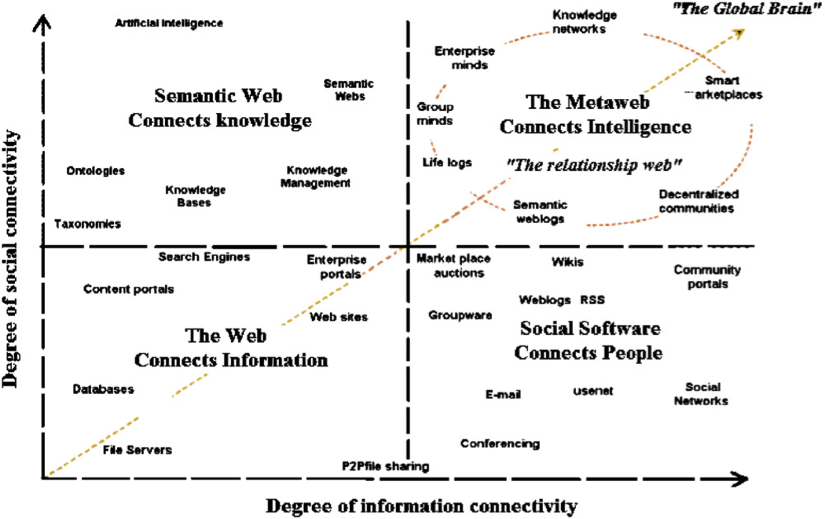
\includegraphics[width=15cm]{bernard.png}
  \caption{A taxonomy for collaboration alternatives \cite{Albors2008}.}
  \label{Figure:figex2c}
\end{figure}

\section{Web 2.0 and Social Media}

Web 2.0 is the term coined by Tim O�Reilly for the new phase of web where not only the technology but also the business revolution in the computer industry is caused by using web as a platform. The main characteristics of the Web 2.0 websites are that it creates object-centred networks where people connect via objects of interest.

The first wave of socialization of Web began with the appearance of blogs and wikis, as it was easier to create content without the knowledge of HTML and web development. The easy to use "What you see is what you get" editor helped creation of large amount of contents and people could communicate and collaborate easily with each other, the original idea of Berners-Lee came into effect when the web was both read and write.

\subsection{Blogosphere}

Services like LiveJournal \footnote{\url{http://www.livejournal.com/}} and Blogger \footnote{\url{www.blogger.com/}}, both started in 1999, created a network of people with similar interest and purpose and create a collaborative knowledgebase for the community of like-minded people. The blogosphere soon recognized as a densely interconnected social network through which news, information, ideas and opinion travel rapidly formed by professional and corporate bloggers as well as hobbyists.
As of 2011, NM Incite studies tracked over 181 million blogs growing from 36 million in 2006 and there are 1 million new posts everyday \cite{nm2011}.

Nowadays, there are blogs in every category and topic and it has turned into the means to share news and information instantly, like the Huffington Post\footnote{\url{http://www.huffingtonpost.com/}}. These blogs are densely interconnected and are networked together based on region, language, topics and categories. Blogs have made it easier for user to create new content and easily share it with the masses. The simple editor does not require any technical knowledge and it is a large-scare platform for people to create network with similar interest and expertise.

\begin{figure}[!htb]
  \centering
  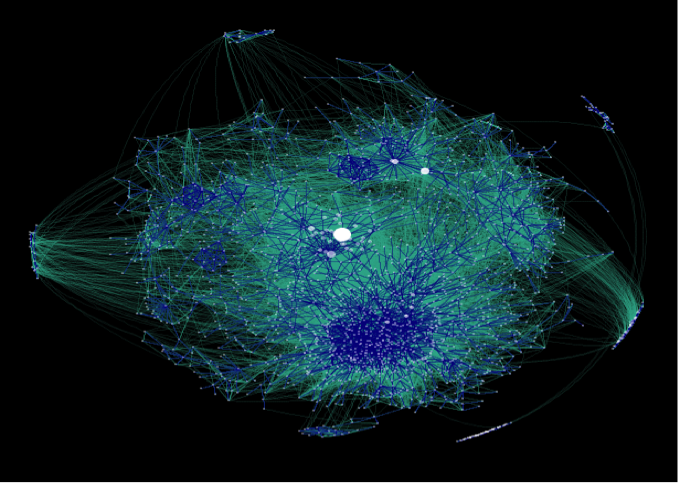
\includegraphics[width=15cm]{blog.png}
  \caption{Blogosphere as social network \cite{hurst2007}}
  \label{Figure:figex2a}
\end{figure}

\subsection{Social Networking Services}

In 2003, one of the earlier social networking website Friendster \footnote{\url{www.friendster.com/}} had attracted 5 million users that created profile and connected with friends and family, soon many other similar website emerged of which Facebook was the most successful with more than 900 million user as of March 2012. People create explicit connect with friends or colleagues (LinkedIn) to communicate and share contents with them.

People use these websites in every aspect of their life, they use it to share personal information with friends and family, use it to share their work and interest with colleagues and play games with other users. Now, business enterprise have also adopted these social networking website to connect to their consumers and advertise the products directly to the people who are interested in it \cite{ridings2004virtual}.

These websites now, not only connect people together through personal connection, it also connects people through shared objects. A good example of this is Facebook 'Like' button, this is used to connect people who like the same music or movies or share similar interest. This creates a vast community of people who share same interest and also share similar information. This giant global graph of people and object connected together is similar to the idea of Linked Data.

\subsection{Microblogging}

There are also microblogging services like Twitter and Tumblr \footnote{\url{https://www.tumblr.com/}}  makes sharing information quicker and faster. These services create implicit relationship between people by follower-following method. The social network grows quickly as people do not need to approve any friendship and the content is distributed widely and rapidly by the re-sharing feature they have. Users can retweet the same tweet in Twitter and reblog the same posts in Tumblr multiple times creating a viral distribution of information.

There are more than 500 million twitter users as on April 2012 and there are 400 million tweets everyday. Analysis of the tweets has suggested that 40\% of the tweets are pointless babbles and only 13\% have some value or important information or news \cite{Whitelaw2011}. The rest of the tweets are spams, conversations or self-promotion and marketing. Twitter and Tumblr allow users to interact, create hash tags and share pictures, videos and other media.

\subsection{Peer to Peer network}

The other method of collaborative information sharing is peer-to-peer network where peers are the computers system connected through Internet. Some software applications like Bit Torrent \footnote{\url{www.bittorrent.com/}}  are used to share any content between the users and large documents can easily be shared by reducing the load on one server. There are many controversy and legal issue with sharing copyright files like music, films and books but this social network allows millions of people to share large amount of data in distributed format.

\subsection{Content Specific Social Networking services}

After Facebook, a new trend emerged for content specific social networking websites like YouTube to watch videos, Flickr to share pictures, Delicious \footnote{\url{http://delicious.com/}}  to share bookmarks, LastFM \footnote{\url{http://www.last.fm/}}  to listen to music, etc. In these websites people connect with other people with similar interest and passion. They form groups and communities and use user participation rate the content for quality control and user behaviour recommendation.

These are open networks where people can upload their content and it is visible to the whole world. It gives a platform to broadcast creative content to the large audience. These networks are completely depended on user contribution to sustain the community.

\section{Collective Intelligence and Crowdsourcing}

The World Wide Web provided a platform for people to share, discuss ideas and information, and collaborate with each other. The Web 2.0 main trend was using the collective intelligence of people to create a knowledgebase, get user preference and do recommendations.

\subsection{Wiki}

Web 2.0 provided easy to use tools for collaborative authoring and ownership of information. A wiki allows users to add, remove, edit or modify any content on a webpage and keep tracks of different versions changes. Wikipedia \footnote{\url{http://www.wikipedia.org/}}, a collaborative encyclopaedia, is an excellent example where people with similar interest and expertise came together to create this vast knowledgebase. Crowdsourcing is used for quality control and to stop vandalism spamming. These collaborative networks strive because they enforce a strong sense of community with people through collaboration and creation of content where individual contribution was counted and it became an efficient knowledge management tool.

\subsection{Folksonomy}

The other feature of Web 2.0 was the ability to add tags to any content and user generated taxonomy is utilized to categorize the pictures, videos, music and every kind of data. The tags make sit easier to classify and categorize information and also to search and discover similar content on any topic. Collaborative tagging and bookmarking is used to add metadata and categories to pictures in Flickr and links in Delicious and it makes it easier for people to search and discover information. Using multiple tags also connects categories and geo-tagging helps in identifying any object based on location.

\subsection{Open Source Software}

Linux open source software project gave an alternative to the traditional software development and the programmers formed a community to build the software and tools. The system provided the developers with a platform to collaborate and create where individual authorship is recognized but they don�t get exclusive intellectual rights. Creative common license is used and it allows the creator to easily mark their creative work and share it with the world.

This type of large-scale software development requires lots of co-ordination and communication with the community and a project is divided into various phases of development. There are many tools available, like version control, bug tracking, task management and testing tools, for people to collaborate and communicate. Many software products like Firefox, Android, etc. are successfully developed and used by general mass.

\subsection{Forums and messaging boards}

Forums and boards gave a place for people to meet anonymously and have a discussion, it was the beginning of virtual community where face to face communication was replaced by messaging boards, chat rooms, question and answer forums. These online communities were formed based on interest and common objective and people from all around the world could come together and communicate on a particular topic of interest \cite{adamic2008knowledge}.

\subsection{User Recommendation system}

The power of collective behaviour and knowledge was utilized by the websites like Amazon \footnote{\url{http://www.amazon.com/}} and Pandora \footnote{\url{www.pandora.com/}} for recommendations of books and music respectively. Users in these websites also rate and review the things and crowdsourcing is used for predicting users� needs and contents can be recommended accordingly.

\subsection{Human Computation}

Humans are good at solving the AI complete problems like natural language processing, image analysis that computers still have problem solving. Luis von Ahn came up with various systems to utilize human computation and use crowdsourcing to solve these problems. The ESP games \cite{vonAhn2004} are used to annotate images on the web \cite{von2006games}, reCaptcha \cite{vonAhn2003} is used to digitize millions of book and Duolingo \footnote{\url{http://duolingo.com/}} is used to translate the web into various languages.

These systems are used by users to play games, identify humans from machines to stop spams, and to learn foreign language and they utilize the tasks easily done by human to solve computational problems. The same task done by many people give a common consensus to knowledge and prevent errors \cite{von2009human}.

\section{Semantic Web and Social Networking}

The idea of a Semantic Web was coined by sir Tim Berners-Lee in his Scientific American article \cite{berners2001semantic} that described it as an extension of the current web, where all data is structured and has a meaning accessible by both machines and people. Linked Data is a set of best practices for publishing reusable structured contents using the existent Web as a sustaining framework. In Linked Data every resource is represented by a URI and HTTP URIs are used in order to retrieve documents that describe those resources. Documents are described with RDF where links to other resources are then used.

There are many Semantic Web technologies and application available in the area of social network and social media. These technologies help with data representation, data portability and cross platform interoperability. Using Linked Data principles a decentralized system can be created that helps in social network integration. Every object and entity is identified using a URIs and it is deferenceable by using HTTP \cite{shadbolt2006semantic}. Also, useful metadata about the entities can be added in structured format using RDF and it could be linked with other related data to improve discovery. Some of the social semantic technologies and application is discussed below.

\subsection{Social Semantic Technology}

As previously discussed there is already a large amount of linked data available on Web called Open Linked Data cloud and there are many useful ontologies to represent this data, including social data. The evolution and formation of different and most widely used ontologies to describe people, communities, and their data are discussed below.

\subsubsection{FOAF}

FOAF ontology is used to describe people and the relationship between them. Each person has a unique identifier and a specific vocabulary is used to create personal profile of the users and describe their social network. It can be easily integrated with other Semantic Web ontologies and a person can describe one or more of their online social network \cite{brickley2010foaf}.

Many websites like LiveJournal, FriendFeed, identi.ca uses FOAF to describe their users. Many other websites has plug-in or external application that create their FOAF profile like FOAF generator, WordPress plug-in etc. It helps to solve distributed identity problem when one user has different account in different website, using FOAF, a user can combine all the information from various sources into one file and interlink his different identity and social network. This also helps in creating a complete user profile and cross-site content recommendation \cite{bojars2008interlinking}.

Privacy and digital identity protection issues can also be resolved in FOAF by using SSL protocol that provides distributed authentication system to different user and create different policy for private and public information \cite{bojars2008weaving}.

\begin{figure}[!htb]
  \centering
  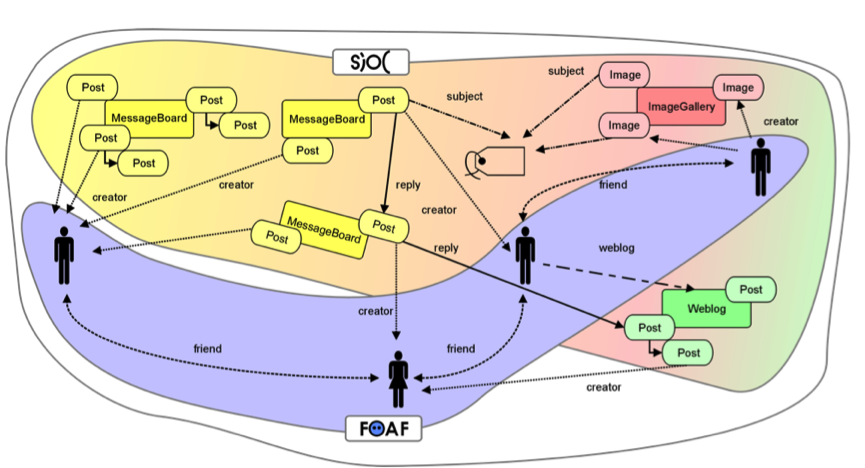
\includegraphics[width=15cm]{foaf.png}
  \caption{Creating a FOAF profile and SIOC file of a user.}
  \label{Figure:figex2b}
\end{figure}

\subsubsection{SIOC}

SIOC ontology is used to describe online communities� activities and interlink them together. It can be easily integrated with FOAF profile of a user, so the combined document contains users� information, their social network and all the data user created with the comments and metadata provided by others \cite{breslin2005towards}.

SIOC can be used for blogs, forums, discussion board, mailing lists, etc. Many websites uses SIOC as well as ma enterprise and E-government uses SIOC to freely available their data.

SIOC is the next step in integrating different social networks together, it describes the content of the website with a structured format so the information is easier to access, search, and discover. The posts can be browsed in many innovative ways by using specialized queries. It creates connection between people from different networks and people with different account can use it with FOAF to prevent identity problems or co-referencing. It makes it easier for people to connect the data in decentralized system ad enable data integration \cite{breslin2007future}.

The above figure describes how FOAF and SIOC together can help interlinking and integrating different communities and different account of the same person together using Semantic Web technology for easy reusability.

\subsubsection{OPO}

The OPO ontology is used to describe the online presence of a user who is using instant messaging service. It stores the state of user, if they are online or offline and who they are communication with and what they are communication.

\subsection{Social Semantic Applications}

Social web and semantic web has come a long way in past ten years. There are many social semantic application available present on the web that solves many underlying problem present in the SNS. They are described below \cite{Gruber2008}.

\subsubsection{Semantic Tagging}

People in Web 2.0 use tags to classify, categorize or group their content using their own vocabulary. This has enabled users to generate more data but this also ambiguous and imprecise.   People use different terms in the same context meaning the same concept and same terms in different contexts for different meanings.

The main issues with tags are the tag ambiguity problem where it is not clear in what context a tag is used. For example if a post tagged with �Apple� is describing a fruit or a computer brand. That�s why is so important to reconcile lexical tags to URIs that unambiguously identify the meaning of a term \cite{garcia2009preliminary}. The same tag actually differs when people use different spelling or space or hyphen between words. And there is also a lack of organization and hierarchy between tags \cite{correndo2007survey}. It is hard to comprehend if a tag marked �Apple� is a subclass of a tag marked �Fruit.�

Most of these problems can be solved by the MOAT ontology that helps to describe the meaning of a tag semantically and connect it with the object and related tags. Also the co-occurrence of tag can be used to group similar tags together. It is user defined interlinking and the contents are linked to the Linked Data Cloud. It uses the collaborative approach to share the meaning of tag in a community.

The Tag Ontology helps to solve the ontological and hierarchical problem that exists between groupings of tags. The SCOT (Social Semantic Cloud of Tags) ontology creates a model to describe a tag cloud and it makes the tag cloud portable so it can be exported from one service to another without losing the data.

Many research is carried out in the area of extracting ontologies from tags, FolksOntology is one of those project that extracts relationships between tags. FLOR is another project that automatically identifies the meaning of a tag. These ontologies can be combined with other ontologies to create a complete model for semantic tagging in the area of social network \cite{bojars2008interlinking}.

\subsubsection{Semantic blogging and microblogging}

Blogosphere is a huge part of the web where people are generating data in exponential rate, but most of this data is not structured or categorized, it is in plain text \cite{chin2006social}. With the advent of Twitter, microblogging is the new trend and this also lacks context and structure.

Semantic web technologies can be used to semantically annotate useful content and keywords of the blog posts and micro blogs to add meaning and structure to it. Drupal \footnote{\url{http://drupal.org/}} website provides an easy to use platform to add annotation to the blog posts and it embeds RDFa into them. Twitter Annotation service takes the tweet metadata of location, time, etc. and annotates them to provide semantic metadata.

Another important project that helps in semantic blogging is the Open Graph Project and Facebook Open Graph that helps users to express preferences increasing in this way the quality of the information provided in the blogs or indeed in any website \cite{rowe2009interlinking}. People can add reviews and ratings to a movie or use the Facebook �Like� button to show their preference and the Open Graph project connects the objects and resources with people, their friends and people with similar interest to provide better recommendation. These projects follow an Open Graph Protocol and create the data in RDF and the data can be queried to provide useful information.

The main use of these technologies is that it is easier for users to publish their data in structured format and they can publish it cross-site because it is portable. The developers can quickly create mash-ups to provide better data visualizations by integrating data from different sites because search and discover is easy in structured data. This data can also be mapped to people�s FOAF profile and SIOC data files. If the dataset has a SPARQL endpoint, querying and retrieval of data can be done \cite{millard2010consuming}.

\subsubsection{Semantic Wiki}

Wiki is an excellent example of collaborative creation and edition for emergent knowledge. There is a large number of people editing Wiki pages and helping in maintaining the quality of the information and preventing spam and irrelevant information \cite{chi2009augmented}. The structured information from the Wikipedia info-boxes has already been converted into linked data within the DBpedia \footnote{\url{http://dbpedia.org/}} project, and this data set is already one of the largest and most linked dataset in the Open Linked Data cloud.

DBpedia is very useful because it uses Wikipedia data and it is easy for anyone to read or write a Wikipedia article, and it also solves the problem machines cannot by using Crowdsourcing. But DBpedia only uses part of the data because Wikipedia lacks proper structure and agreed semantics of the data and its categories. This problem can be solved by semantic wiki where all the data is structured and properly categorized. This provides better search and discovery of information like in OntoWiki \cite{Albors2008}.
%% ----------------------------------------------------------------
%% PSN.tex
%% ---------------------------------------------------------------- 


\chapter{Purposive Social Network} \label{Chapter:Purposive Social Network}
Hello

\section{What is Purposive Social Network}
\subsection{Information Based Community}
\subsection{Interest Based Community}
\subsection{Expert Based Community}
\subsection{Location Based Community}

\section{Characteristics of Purposive Social Network}
\subsection{Community Size}
\subsection{Focused Interest}
\subsection{Direct Communication}
\subsection{Active Participation}
\subsection{Short Lifespan}
\subsection{Strong Incentive}

\section{Benefits of Purposive Social Network}
\subsection{Information Exchange and Self-interest}
\subsection{Symbiotic Relation and Social Exchange}
\subsection{Social Recognition and Personal Satisfaction}
\subsection{Recommendation System}
\subsection{Expert Finder}

\section{Crowdsourcing in Purposive Social Network}
\subsection{Recruiting and Retaining Users}
\subsection{Incentive Model}
\subsection{Quality Control}
\subsection{Search and Discovery of Quality Content}

\section{Use of Semantic Web and Linked Data in Purposive Social Network}
\subsection{Structured Data}
\subsection{Linking People to People and People to Data}
\subsection{Multidimensional Network and Graph}
\subsection{Integrated Knowledgebase}
\subsection{Smart Query and Search}
\subsection{Social Network Analysis}
%% ----------------------------------------------------------------
%% Analysis.tex
%% ---------------------------------------------------------------- 


\chapter{Analysis of Purposive Social Network} \label{Chapter: Analysis of Purposive Social Network}

A purposive social network is a broad and general concept that can be applied to many different social networks. At its core, it is a network with a specific goal and purpose where people come together to solve a particular problem.

For this research StackOverflow website is analyzed where programmers and developers ask questions and experts in the field answer them and solve the problem. In this analysis, the user asking and answering questions, voting the responses and commenting are the main entities of the social network. Their network ties are measured by their communication and interaction between them. The amount of their contribution is measured by the crowdsourcing where people give up votes or down votes to their posts and the badges they receive for their contribution.

\section{Network Linkage and Social Ties}

StackOverflow is not a typical social networking website per se as users cannot create an explicit friendship or follow other people�s work, they cannot send private messages or form groups.

The social ties are form implicit by user interaction with each other through asking questions and answering them, voting on the posts and commenting on them. The communication network is studied to see the social ties of the individuals \cite{monge2003theories}.

\begin{table}[!htb]
  \centering
  \begin{tabular}{cc}
  \toprule
  \textbf{Post Type} & \textbf{Number}\\
  \midrule
   Questions & 3279233\\   \midrule
   Answers & 6578079\\   \midrule
   Registered Users & 1225580\\   \midrule
   Tags & 30408 \\   \midrule
   Unanswered Questions & 780535\\   \midrule
   Badges & 3454994\\   \midrule
   Votes & 26184363\\   \midrule
   Comments & 12526162\\ 
  \bottomrule
  \end{tabular}
  \caption{StackOverflow at glance as of June 2012}
  \label{Table:tabex}
\end{table}

As of June 2012, there are over one million registered users in StackOverflow and more than 3.2 millions questions asked by users. The questions are categorized using tags and individual users can subscribe to tags to receive daily email of all the question asked in the tag. There are more than 30 thousand tags associated with various questions and answers. Users have casted more than 26 million votes to mark the good questions and answers.

\begin{figure}[!htb]
  \centering
  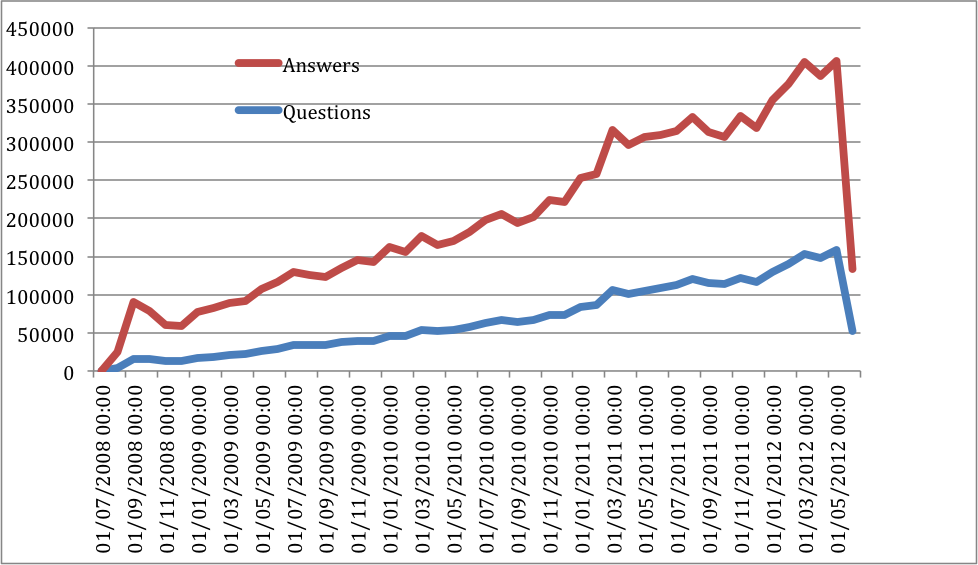
\includegraphics[width=15cm]{qa.png}
  \caption{Questions and answers posted per month on StackOverflow}
  \label{Figure:figex4a}
\end{figure}

The \fref{Figure:figex4a} shows the number of questions asked and answered by users each month. In the year 2012, each questions have on average 1.645 number of answers.

This community is made of programmers and their motivation is to solve the problem they had encountered and to provide answers to gain reputations. Thousands of questions and answers are posted everyday. The analysis of posts shows that the programmers prefer to ask the questions and answers on weekdays.

\begin{figure}[!htb]
  \centering
  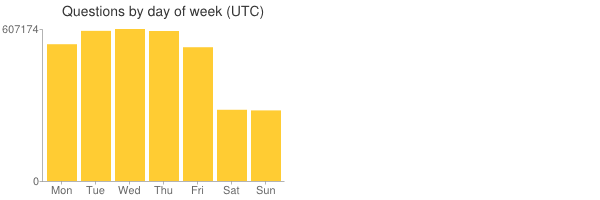
\includegraphics[width=15cm]{chart1.png}
  \caption{Questions posted by the day of week}
  \label{Figure:figex4b}
\end{figure}

Despite high user feedback and participation, 23.79\% of questions are not answered or the answers do not receive any up votes. On average a question receives 2.006 answers and .12\% of questions receives more than 15 answers.

\begin{figure}[!htb]
  \centering
  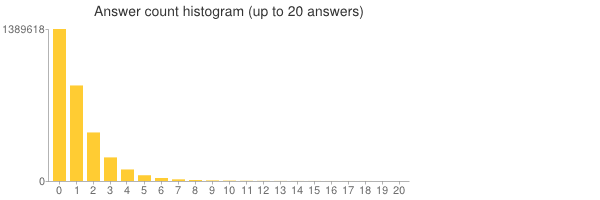
\includegraphics[width=15cm]{chart2.png}
  \caption{Answer count to the questions}
  \label{Figure:figex4c}
\end{figure}

The questions are answers are provided with tags to categorize and arrange for easy search and discovery. The entire website is categorized using the tags and the list of most popular tags are shown in the table. The figure shows the weekly use of the popular tags. The number of questions asked for each tags also provides an insight on the popular language used by developers at the time.

\begin{table}[!htb]
  \centering
  \begin{tabular}{cc}
  \toprule
  \textbf{Tags} & \textbf{Number of instance}\\  \midrule
   C\# & 370074 \\ \midrule
   JAVA &  315488 \\ \midrule
   PHP & 293755 \\ \midrule
   JavaScript & 278592 \\ \midrule
   Android & 244791 \\
  \bottomrule
  \end{tabular}
  \caption{Five most popular tags and its instances}
  \label{Table:tabex2}
\end{table}

\begin{figure}[!htb]
  \centering
  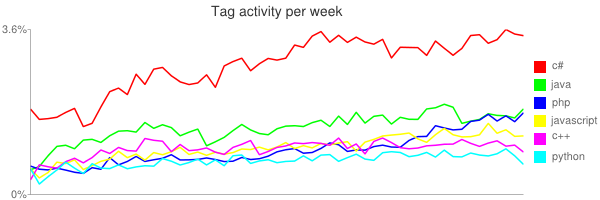
\includegraphics[width=15cm]{chart3.png}
  \caption{Tag trends per week of most popular tags}
  \label{Figure:figex4d}
\end{figure}

The analysis of questions shows that each question has between one to five tags associated with it. Most questions (70.30\%) have 2 to 4 tags associated with it. The relationship between the tags shows the overlapping of networks and how it is tied with one another.

\cite{Eberhardt2012} provided an interactive graph in his website to show the relationships between the most popular tags and how closely they are related to each other. In the following graph each segment size is directly proportional to the number of instance it is used and the connection between the tags indicate the times they have been used together in a question. The thickness of the connection shows the strength of the relations. The segment is colour coded by the frequency of connections, red segments are strongly connected and blue segments are weakly connected.

\begin{figure}[!htb]
  \centering
  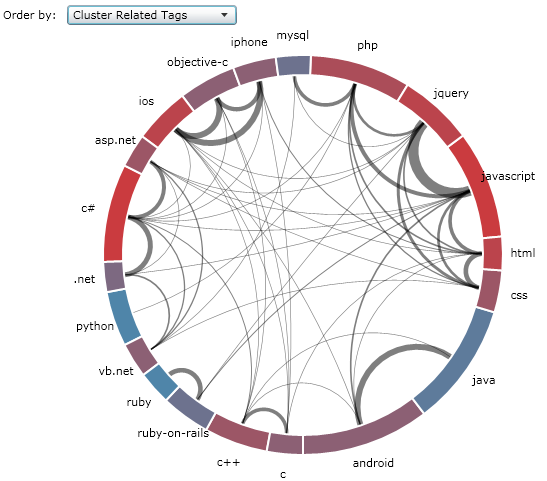
\includegraphics[width=11cm]{graph1.png}
  \caption{Related tags clustered together}
  \label{Figure:figex4e}
\end{figure}

\begin{figure}[!htb]
  \centering
  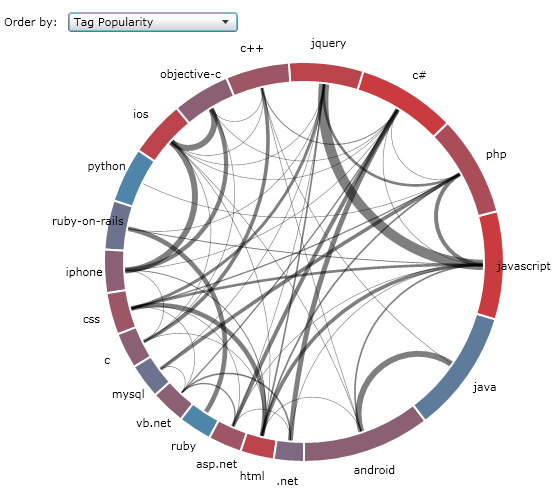
\includegraphics[width=11cm]{graph2.png}
  \caption{Popular tags clustered together}
  \label{Figure:figex4f}
\end{figure}

The clustering of the tags shows the relationship between the tags and technologies. The two popular tags JAVA and Android are closely related to each other but are scarcely joined with other tags. The strongest relationship is between jQuery and JavaScript because the overlapping framework of the two programming languages. C, C++ and C\# are also a closely related groups as well as iOS, Objective-C and iPhone. However, sometimes Objective-C is also tagged with C, C++ and C\#, if by mistake or deliberately can be argued.
There is a large cluster of connected web development languages, CSS, HTML, JavaScript and jQuery, indicating the close knit use of these technologies in development of website and web applications. The interesting thing is the relationship between the scripting langue PHP and Python, they are popular tags but are sparsely connected with other tags and are weakly linked with database related tags.

\section{Role of Individual Actors}

Users who contribute to the website are the main actors of this purposive social network. There are more than 1.2 million registered users in StackOverflow and they ask the questions, answer it, vote it and moderate the community. The users are not directly linked to each other to create relationships; in this network the relationship is formed by their interaction and their contribution. The user behaviour, their motivation to use the website and incentive to contribute is described below.

Despite the high content generation by the users, 56.02\% do not interact or contribute to the website, they have 1 reputation point that they receive while joining the website.

\begin{figure}[!htb]
  \centering
  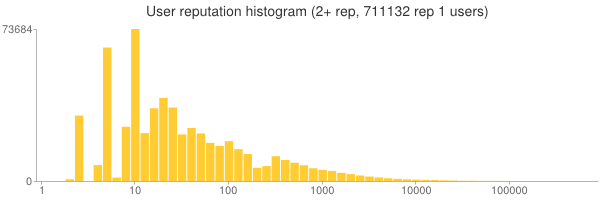
\includegraphics[width=15cm]{chart4.png}
  \caption{User reputation histogram}
  \label{Figure:figex4g}
\end{figure}

\begin{table}[!htb]
  \centering
  \begin{tabular}{cc}
  \toprule
  \textbf{Reputation} & \textbf{Number of users}\\  \midrule
  1 & 669554\\ \midrule
  2-10 & 126235\\ \midrule
  11-100 & 295389\\ \midrule
  101-1000 & 3161130\\  \midrule
  1001-10000 & 170993\\ \midrule
  10001-20000 & 1437\\ \midrule
  20001-100000 & 895\\ \midrule
  100001-200000 & 49\\ \midrule
  less than 200000 & 11\\
  \bottomrule
  \end{tabular}
  \caption{Number of users with reputations}
  \label{Table:tabex3}
\end{table}

As \tref{Table:tabex3} shows, there are 669554 users with 1 reputation point and one user with 452951 reputation points. The distribution of the users reputation shows that more than half of the users are lurkers and the elite users with the most reputation points are the editors and moderators of the community and are considered the expert in their field.

The reputation of the user has a direct correlation with the trust in the community. StackOverflow has designed an excellent reward program to motivate and incentivize the users to contribute and gain more reputations and badges.

Currently, there are 77 different types of badges given to the user based on their contribution. There are badges given to the user who asks questions with 1 reputation point (Student), to the user who edits the answers to make posts better (Editor) and to even an active user for a year (Yearling). This type of virtual acknowledgement of efforts encourage the user to participate and contribute to the website.

The other method that encourages the users to participate is the promptness of the response. The asker prefers to receive information sooner rather than later, and will stop the process when satisfied with the cumulative value of the posted information. The analysis of the posts shows that half of the questions get an answer within an hour of the posting and within a day the questions receives an accepted answer. When the answers are delayed, the questioners look for alternative websites to get a response.

\begin{figure}[!htb]
  \centering
  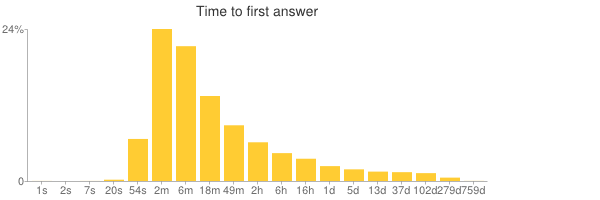
\includegraphics[width=15cm]{chart5.png}
  \caption{Time to receive the first answer}
  \label{Figure:figex4h}
\end{figure}

\begin{figure}[!htb]
  \centering
  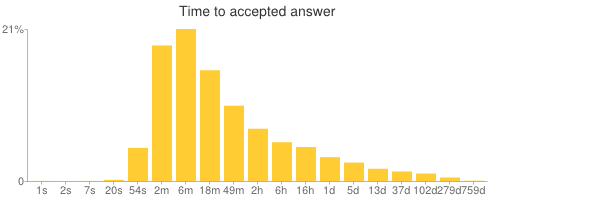
\includegraphics[width=15cm]{chart6.png}
  \caption{Time to get the accepted answer}
  \label{Figure:figex4i}
\end{figure}

\section{Incentive Design and Quality Control}

The StackOverflow website uses a game theoretic model to encourage user participation and activity. Participation is encouraged through an elaborate point system and users also receive badges for participation. Also, the top contributor and user with highest reputation are featured on the question page, giving the user more visibility and acknowledgement of the user�s expertise. This encourages participants to accumulate more points and contribute to get recognition.

When an answer is votes up, the user gains 10 reputations and 5 points when the question is voted up. When an answer is accepted the user receives 15 points and there is also negative point system, a user looses 2 reputation point when a question or an answer is voted down. This keeps the spamming in check and repeated questions and answers are avoided.

The system also encourages users to participate as the higher reputation points gain more privileges. When a user has 15 reputation points, only then they can up vote and 50 points allows users to comment. To stop harassment and spam, user requires 125 reputation points to vote down and it costs the user 1 reputation point. The incentive model is thorough and higher reputation points open more gates for users to interact and contribute and be acknowledged as the expert in their field.

The community thrives because of the high quality of content and it is possible by the user�s action and moderation. Users vote up the good questions and answers and vote down the bad quality content or repeated posts. There is more than 6 million votes casted in the website and the user with enough reputations are allowed to cast 40 votes per day.

\begin{figure}[!htb]
  \centering
  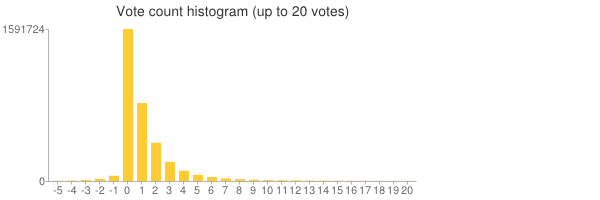
\includegraphics[width=15cm]{chart7.png}
  \caption{Vote count histogram}
  \label{Figure:figex4j}
\end{figure}

\begin{table}[!htb]
  \centering
  \begin{tabular}{cc}
  \toprule
  \textbf{Vote} & \textbf{Vote Count}\\  \midrule
  less than 20 & 25\\  \midrule
  0 & 504754\\  \midrule
  1-10 & 7802690\\  \midrule
  11-100 & 718650\\  \midrule
  101-1000 & 6460\\  \midrule
  1000-5000 &11\\
  \bottomrule
  \end{tabular}
  \caption{Questions� votes count}
  \label{Table:tabex4}
\end{table}

The analysis of the questions and votes shows that every question receives 3.06 votes on average. One question received negative 115 votes and the highest vote received to a question is 2499. Similar analysis of answers and their votes shows that, on average an answer receives 0.99 votes and the lowest vote to an answer is negative 57 and the highest vote is 4432.

\section{Using Semantic Web Technologies}

The data extracted from StackOverflow website is in the form of simple text, some of the posts contain HTML codes but they are snippets of code and are represented as text in the database. The users categorize the posts by using tags and it gives information about the topic and the programming language the question is being asked. The answers do not have special tags but the tags of the questions are applied to the answers as well.

\subsection{Using RDF and Linked Data}

All the user data, post data, votes and badges are transformed in RDF data by applying simple RDF schema and ontologies.

The website only shows basic user profile information due to the privacy reasons and FOAF ontology is used to describe the data. An example of the simple user profile information is as follows:

\begin{verbatim}
<foaf:Person>
    <foaf:name> Geoff Dalgas </foaf:name>
    <foaf:mbox_sha1sum> b437f461b3fd27387c5d8ab47a293d35 </foaf:mbox_sha1sum>
    <foaf:based_near> Corvallis, OR </foaf:based_near>
    <foaf:age> 35 </foaf:age>
    <foaf:OnlineAccount> http://stackoverflow.com/users/2/geoff-dalgas 
    </foaf:OnlineAccount
</foaf:Person>
 \end{verbatim}
 
 Similarly, the posts created by users, the questions and answers are described using SIOC ontology. The content is described and linked with the user RDF using the similar URIs.
 
\begin{verbatim}
<sioc:Post rdf:about=" http://stackoverflow.com/questions/89228/calling-an-external
-command-in-python">
    <dcterms:title>Calling an external command in Python</dcterms:title>
    <dcterms:created> 2008-09-18T21:42:52.667 </dcterms:created>
    <sioc:has_container rdf:resource=" http://stackoverflow.com/questions/tagged
    /python"/>
    <sioc:has_creator>
       <sioc:UserAccount rdf:about=" http://stackoverflow.com/users/170339/bludger " 
       rdfs:label="bludger"> </sioc:UserAccount>
     </sioc:has_creator>
     <sioc:content>How can I call an external command in Python</sioc:content>
     <sioc:topic rdfs:label="python" rdf:resource=" http://stackoverflow.com
       /questions/tagged/python"/>
     <sioc:topic rdfs:label="command" rdf:resource=" http://stackoverflow.com
       /questions/tagged/command"/>
     <sioc:has_reply>
        <sioc:Post rdf:about=" http://stackoverflow.com/a/89243/1313327">
            <sioc:content>Look at the subprocess module in the stdlib: from subprocess 
             import call call(["ls", "-l"]) The advantage of subprocess vs system is that 
             it is more flexible (you can get the stdout, stderr, the "real" status code, 
             better error handling, etc...). I think os.system is deprecated, too, or will
             be: http://docs.python.org/library/subprocess.html#replacing-older-functions
             -with-the-subprocess-module For quick/dirty/one time scripts, os.system
             is enough, though.</sioc:content>
             <dcterms:created>2008-09-18T23:42:52.667</dcterms:created>
             <sioc:has_creator>
                <sioc:UserAccount rdf:about=" http://stackoverflow.com/users/11465
                 /david-cournapeau" rdfs:label=" david-cournapeau "> </sioc:UserAccount>
              </sioc:has_creator>
           </sioc:Post>
      </sioc:has_reply>
</sioc:Post>
\end{verbatim}

\subsection{Topic Disambiguation}

The StackOverflow dataset is sparsely annotated by user-generated tags and it is not linked with any other datasets. When user creates a question, they add tags to it to categorize into different topics but the answers have the tags from the questions. Also, all the main topics inside the text of question or answer is not clearly stated. The topics are ambiguous and not linked to any vocabulary or properly annotated.

A sample of the question, answer and tag data is annotated with the links from Wikipedia datasets and Drupal datasets to resolve the name and topic disambiguation. These services do the name entity recognition and match the entities with the appropriate topics and categories. The service does not convert the text into Linked Data or RDF, the returned data is further transformed into RDF and linked with the DBpedia dataset.

Wikipedia Miner service is used to annotate a small sample of posts, the service returns the text with annotated topics embedded into the text. The service accepts simple text or HTML and one can specify the density of links to be added and the level of accuracy required from the service. Below is an example annotated text of a question and answer posted.

\begin{figure}[!htb]
  \centering
  \subfigure[Annotating a text question]{
    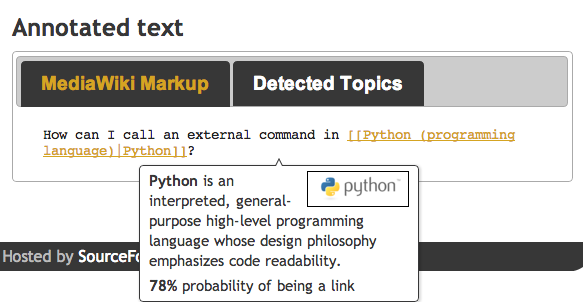
\includegraphics[width=14cm]{q.png}
    \label{Figure:figsubex11:left}
  }
  \subfigure[Annotating a text answer]{
    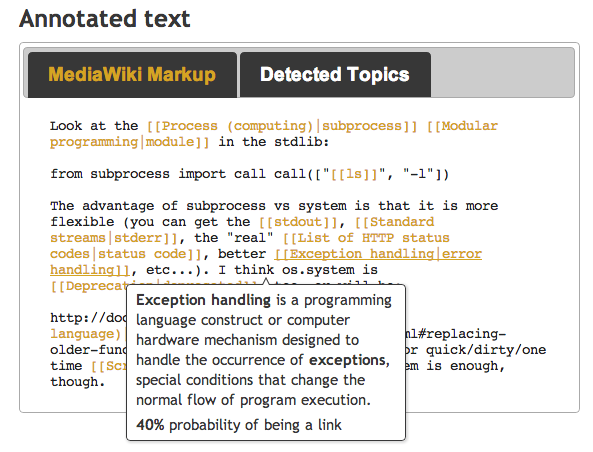
\includegraphics[width=14cm]{ans.png}
    \label{Figure:figsubex11:right}
  }
  \caption{Wikipedia Miner web service annotating a text question and an answer}
  \label{Figure:figsubex11}
\end{figure}

The Wikipedia miner service uses a word sense disambiguation based machine learning algorithm and where it detects key terms in a text excerpt and disambiguating then against Wikipedia article. It provides a JAVA API to access the Wikipedia database, including all the categories and it can be searched, browsed and iterated over \cite{milne2012open}.

OpenCalais is another web service used to annotate the StackOverflow posts with the Drupal dataset. This tool creates a semantic rich metadata for the content using the natural language processing, machine learning and name disambiguation algorithm. It provides many services; it provides tag integration with different taxonomy and vocabulary, geo-mapping of location and semantic annotation of keywords. An example annotation of text using OpenCalais is below.

Text sample question: "Does Python have a ternary conditional operator? If not available, is it possible to simulate one concisely using other language constructs?"

\begin{verbatim}
<SocialTags>
  <SocialTag importance="2"> Conditional
	<originalValue>Conditional (programming)</originalValue>
  </SocialTag>
  <SocialTag importance="2"> Python
  	<originalValue>Python (programming language)</originalValue>
  </SocialTag>
  <SocialTag importance="2"> C
  	<originalValue>C (programming language)</originalValue>
  </SocialTag>
  <SocialTag importance="2"> Ternary operation
  	<originalValue>Ternary operation</originalValue>
  </SocialTag>
  <SocialTag importance="1"> Software engineering
  	<originalValue>Software engineering</originalValue>
  </SocialTag>
  <SocialTag importance="1"> Computing
  	<originalValue>Computing</originalValue>
  </SocialTag>
  <SocialTag importance="1"> Computer programming
  	<originalValue>Computer programming</originalValue>
  </SocialTag>
</SocialTags>
\end{verbatim}

As seen from above snippet, the OpenCalais service finds the keywords and matches it with a taxonomy or vocabulary and assigns the importance to the tag that it is disambiguating.

Both the services do the name entity recognition and match it to a known vocabulary and taxonomy. They do a natural language processing of the text and annotate the keywords. This annotation is then matched with the Wikipedia topics and the StackOverflow data is linked to the Wikipedia data.

These links when analyzed tell the type of categories the keywords matched to give additional information that the StackOverflow tags do not provide. The analysis shows the most asked question is asked from the following categories of programming languages:

\begin{table}[!htb]
  \centering
  \begin{tabular}{cc}
  \toprule
  \textbf{Annotated keyword} & \textbf{StackOverflow Tags}\\  \midrule
  Programming Language & C\#, JAVA, Python\\ \midrule
  Framework & jQuery, ASP.net\\ \midrule
  Environment & Android, iPhone\\ \midrule
  Database & MySQL, SQLite\\
  \bottomrule
  \end{tabular}
  \caption{Keyword analysis of StackOverflow question tags}
  \label{Table:tabex5}
\end{table}

It can be seen from the above example, name entity recognition, creating vocabulary and matching the keywords to a topic and linking it to another knowledgebase provides additional information. This leads to better search and discovery of information and using this an expert in a particular field can also be determined. JAVA being a programming language is also an Object Oriented language and the expert of JAVA also has a good grasp of Object Oriented programming concept and hence can help users in both the scenario.

\subsection{Expert Finder}

According to the StackOverflow website the top user or an expert of C\# is Jon Skeet with more than eighty thousand reputation points and Python is Alex Martelli with more than nineteen thousand reputation point. These users appear on the individual pages of the tags as the top users and without the tag disambiguation they only appear as an expert on a particulate tag, not the joint concept of the topic.

\begin{table}[!htb]
  \centering
  \begin{tabular}{cc}
  \toprule
  \textbf{Tag} & \textbf{Top User with reputation point}\\  \midrule
  C\# & Jon Skeet (80.6k)\\ \midrule
  Java & Jon Skeet (39.7k)\\ \midrule
  Python & Alex Martelli (19.8k)\\ \midrule
  PHP & Pekka (9k)\\ \midrule
  Javascript & CMS (12.3k)\\ 
  \bottomrule
  \end{tabular}
  \caption{Top users of top tags in StackOverflow}
  \label{Table:tabex6}
\end{table}

When the tags are disambiguated and the keywords are matched to the topics, both Java and C\# is categorized at the Object Oriented programming language and here Jon Skeet is considered as an expert in the whole area with more than one hundred and twenty thousand reputation points. Similarly, when the programming languages are further categorized as server side script ion language with Python, PHP and Perl as main languages, Alex Martelli is considered as an expert and the user CMS is expert in the clients side languages such as Java and AJX with twelve thousand reputation points.

\begin{table}[!htb]
  \centering
  \begin{tabular}{cc}
  \toprule
  \textbf{Disambiguated Keywords} & \textbf{Top User with reputation point}\\  \midrule
  Object Oriented programming (C\#, Java) & Jon Skeet (120.3k)\\ \midrule
  Programming language(C\#, Java, Python) & Jon Skeet (120.7k)\\ \midrule
  Server side Scripting language (Python, PHP, Perl) & Alex Martelli (20.2k)\\ \midrule
  Clientside Scripting language (Javascript, AJAX) & CMS (12.3k)\\ 
  \bottomrule
  \end{tabular}
  \caption{Top users of top disambiguated topics in StackOverflow}
  \label{Table:tabex7}
\end{table}

Semantic web and linked data helped in topic  recognition and disambiguation and experts in broader concept and also specialized field can be ascertained even though these information is not present in the main website. The \tref{Table:tabex7} only shows the experts in StackOverflow domain, when the data from multiple website and question/answer forums are combined, the linked data can help find experts in across domain in bigger set of users and help in better search and discovery of experts and information.
%% ----------------------------------------------------------------
%% Conclusions.tex
%% ---------------------------------------------------------------- 


\chapter{Conclusions} \label{Chapter: Conclusions}

Social interaction and creating a social network is part of human nature, we can find the network by studying their communication process. World Wide Web has not only made it easier and simpler for people to connect and interact, it has also made it easier to study these networks. 

People not only connect to their friends and families, they also interact with strangers from all over the world, they create a network and community with people with similar interest and expertise. They use the community to solve their problems and web has provided a platform for this. Forums and question-answering systems have made it easier for them to create a network, share their problems and queries and seek solutions for their problems. This community and system is defined as Purposive social network in this thesis.

This chapter summarises the research question, the findings and research contribution.

\section{Summary of Research}

In this thesis different types of social networking services available in the Web is analyzed and the motivation of creating communities is seen. In the current web, an agile approach is taken to create a network of people based on a topic and interest. People come together with common purpose and solve problems and create purposive social network. This network is small, agile and thrives on the user contribution. Different types of crowdsourcing system are also described where people come together to solve problems and create a knowledgebase. This type of system requires a strong framework to support engagement and incentive for people to contribute.

\subsection{Limitation of current systems}

The main limitation of these websites are that they are closed and users have to create multiple accounts across different websites to use their services. There is no proper way to merge different social network and knowledgebase together. People are stuck in a silos and they don�t have freedom to move to different network and take their data and network with them. 

In this thesis technology based and forums and question-answering system is studied. They are StackOverflow, a question and answer forum where programmers ask questions about their problems and errors and experts in the field answer them and provide solutions. Another website used for research is the programming communities of Reddit. People can ask questions as well as share current news and other information. These websites use crowdsourcing to find the best questions, answers and resources. Crowdsourcing is used to maintain the quality of the content, to moderate the community and to stop spams and other antisocial activities.

These website are quite popular and lots of people post questions and many of the questions goes unanswered or do not have any comments and solutions. The people in the long tail do not get any response. Normal search can be performed and different search engines can be used to look for answers for these questions but they use text search to find solutions and can�t access data from closed system. Also, these search engines don�t use the network structure or other crowdsourcing methods to find answers or experts that can help with solving the problem.

\subsection{Research Question}

In this thesis it is studied to see if Linked Data and Semantic Web technology can be used to find answers for these unanswered questions. These technologies can be used to get different concept and categories of questions and can provide broader search terms to overcome these issues. Also, the social network of the community can be studied and user model can be generated to find experts in the area and they can be recommended to get answers for the unanswered questions. It could improve the long tail of users who don�t find solutions for their questions.

\sybsection{Research Contribution}

StackOverflow and Reddit websites are used to collect the data. A system is created to use the APIs of the website and collect questions, answers, posts, votes and user profiles. The data is analyzed to see the structure of the community, the network is not form by explicit connection of users but by studying the user interaction and how the knowledge is connected with each other. The network ties, user interaction and the incentive model is studied to see how the website with a small community of programmers created a self-sustaining environment for user to participate and continuously create high quality questions and answers and solve problems.

The system also converts the data of top 10 programming languages into RDF. It cleans the data and add ontology and metadata and structures the data collected. It then uses Wikipedia miner and Open Calais tools to annotate the dataset with keywords, solve the name-entity disambiguation problem. These tools perform a natural language processing on the text and uses machine learning algorithm to match the name with Wikipedia topic and Drupal vocabulary. The keywords and topics are categorized and linked with Dbpedia and Drupal knowledgebases and link the data to Linked Data Cloud.

The system also creates a document and keyword frequency matrix to improve the search. This matrix links the questions with keywords as well as keywords with all the questions, answers and experts linked with. These links are also weighted by the votes given to questions, answers and the frequency of the keywords. The data is used to improve the indexing of the database and SPARQL search results. 

To evaluate the system, unanswered questions from the system are used as search query and the answers are saved. The system also recommends experts that are best suited to answer the question. An experiment is designed where people were shown the keywords and answers and asked to rate the quality of the search result.

Statistical analysis is done on the experiment result and it shows that the keyword generated by the system is better than the tags given to the original website data. It also shows that the people agree with the algorithm rating for answers provided by the system.

The system helps to answers the research question and shows that Semantic web technologies and Linked Data can be used to solve the data integration problem of the current web and can be used to integrate heterogeneous systems. The added semantic and linking of the data can help improve the search for unanswered questions in the PSN system that are overwhelmed by number of posts and don�t have answers for all the questions. Semantic Web and Linked data provide a decentralized platform where user generated knowledge can be utilized, improved and help make a community better. It can also recommend experts to create a community for a particular purpose and solve problems. The system provides a platform to integrate different forums and purposive social network to improve the long tail of users that do get the help they ask from the websites.

\section{Limitation of System}

The system helps to show the utility of Linked Data to solve the PSN problem but it has it�s limitation. The system uses the StackOverflow and Reddit data and uses their crowdsourcing data to get the information about the question and answer quality. Any limitation of the original website data is the limitation of the system too. If the user of StackOverflow and reddit stop giving the votes or if the website is filled with spammers then the current system won�t be able to mitigate the situation.

The system uses external tools like Wikipedia Miner and OpenCalais to annotate the text and find the best match for DBpedia and Drupal topics to link. Any limitation of these tools are limitation of the system. Even though the system only accepts keywords and links that have confidence score greater than 50\%, still sometimes the keywords are linked to the incorrect concepts. Also, if there are no Wikipedia or Drupal article for any concept, then those keywords are ignored by the system, even though they are valid keywords.

Currently, the system doesn�t have a user interface. It uses the websites unanswered questions as search terms. So users can�t ask their own questions to search for answers and similar questions. Also, lack of user interface also doesn�t use the crowdsourcing technology to rate the quality of the search result. These limitations can be improved in the future by adding a top layer over the search algorithm that uses crowdsourcing to improve to rate the quality of the system.

The Expert Finder application of the system is not evaluated by the people in the experiment. There was no easy and simple way to provide a complete user profile of every user to the people in experiment and then ask them to rate the expert recommender. Although, the same algorithm that is used to improve the search of answers is used to search for experts. But the experiment result to evaluate the search algorithm for answers can�t be extended to the experts.

The search engines like Google, Bing, etc. use quite sophisticated text search and pagerank algorithm. They crawl the entire webs and find the best match for the search result. Due to limited resources the system only uses two website and provide answers from those dataset. But this was proof of concept, this result doesn�t say the system provides better result than the current search engines.

\section{Future Work}

The system currently does not have any user interface, as said earlier in the limitation, a user interface will let people enter their own questions and help in finding similar questions and answer from StackOverflow and Reddit. Also, another layer of crowdsourcing on top of the system will allow users to upvote and downvote the answers and improve the search result.

Currently, system recommends experts that are best suited to answer the question. The system could be extended to create community and a agile purposive social network. People can use the system to find the right experts to solve their problem, get details of the experts and contact them. The system will get better by adding more communities and website data to the knowledgebase. People can create a agile PSN and find people on different communities and thus extend their own social network.

Currently, the system uses external tools for data annotation to find important topic and categories and link it to the Linked Data cloud. There are research going on deep learning techniques in Natural Language Processing that helps in finding deeper semantics, synonyms and categories to the text. This layer could be on top of the annotation layer. The extracted keywords and extra information from the deep learning algorithms might not be linked to the Linked Data Cloud but it would certainly improve the document keyword matrix. This would improve the overall search results and help find better question and answers in broader and narrower topics.

The system will get better the more dataset it has and knowledgebase it is linked to as it provides a tool for data integration across platforms and it is possible to create a unified knowledgebase from different networks of web communities. Some of the data in the web is freely available but most of the data is still bound behind the closed walls of different websites. Using the APIs of the websites and with the proper encouragement and initiative of users, they can free their own data. These different knowledgebase can be integrated using the semantic web technologies and can be linked with the Linked Data Cloud and improve the community experience.
\appendix
%% ----------------------------------------------------------------
%% AppendixA.tex
%% ---------------------------------------------------------------- 


\chapter{Stuff} \label{Chapter:Stuff}
The following gets in the way of the text....

\backmatter
\bibliographystyle{apalike}
\bibliography{ECS}
\end{document}

%% ----------------------------------------------------------------
